\documentclass[12pt,number,sort&compress]{elsarticle}

%======================================================================
\usepackage{todonotes}
\usepackage{graphicx}
\usepackage[binary-units]{siunitx}
\usepackage{gensymb}
\usepackage{amsmath}
\usepackage[version=3]{mhchem} % Formula subscripts using \ce{}, e.g., \ce{H2SO4}
\usepackage{booktabs,multicol} %better tables
\usepackage{subcaption} %subfigs
\sisetup{group-separator={,},
	detect-all,
	binary-units,
	list-units = single,
	range-units = single,
	range-phrase = --,
	per-mode = symbol-or-fraction,
	separate-uncertainty = true,
	multi-part-units = single,
	list-final-separator = {, and }
	%    scientific-notation = fixed
}
\usepackage[breaklinks=true, linkcolor=blue, citecolor=blue, colorlinks=true]{hyperref}
% load after hyperref
\usepackage[english,capitalise]{cleveref}

%======================================================================
% Add your bibliography file here, replace template.bib
\bibliographystyle{elsarticle-num}

\newcommand{\pluseq}{\mathrel{{+}{=}}}
\newcommand{\minuseq}{\mathrel{{-}{=}}}
\newcommand{\ns}{N_{sp}}
\newcommand{\nr}{N_{reac}}
\newcommand{\conp}{CONP}
\newcommand{\conv}{CONV}
\newcommand{\dconp}{\ifmmode\text{for \conp,}\else for \conp,\fi}
\newcommand{\dconv}{\ifmmode\text{for \conv,}\else for \conv.\fi}
\newcommand{\Ru}{\mathcal{R}}


\title{SIMD\slash SIMT-vectorized Thermo-chemical Source Term Evaluation}

\author[1]{Nicholas Curtis\corref{corr}}
\ead{nicholas.curtis@uconn.edu}
\author[1]{Chih-Jen Sung}

\address[1]{Department of Mechanical Engineering, University of Connecticut, Storrs, CT 06269, USA}
\cortext[corr]{Corresponding author}

\begin{document}

\begin{frontmatter}

%====================================================================
\begin{abstract} % not to exceed 200 words
A code generation platform for single-instruction, multiple-data (SIMD) and single-instruction, multiple thread (SIMT) vectorized thermo-chemical source term evaluation was developed and validated against Cantera for a wide range of chemical kinetic models.
Speedups of up to \SIrange{1.90}{2.45}{$\times$} were observed over a baseline single-instruction, multiple-thread (SIMT) parallelized code.
Additionally, use of a row-major data layout was found to increase both the SIMD and SIMT performance by up to \SIrange{2.00}{2.38}{$\times$} over a column-major data layout.
Larger vector-widths were found to produce speedups up to \SI{1.8}{$\times$} as compared to a small vector-width for smaller models, e.g. GRI-Mech 3.0, but as the model size increased the performance of all vector-widths were similar.
Finally, the parallel scaling efficiency was found to be slightly better for larger models, and future extensions of this work were discussed.
\end{abstract}

% (Provide 2-4 keywords describing your research. Only abbreviations firmly
% established in the field may be used. These keywords will be used for
% sessioning/indexing purposes.)
\begin{keyword}
    Chemical Kinetics\sep SIMD\sep SIMT\sep Vector Processing\sep Jacobian
\end{keyword}

\end{frontmatter}

%====================================================================
\section{Introduction}
%

Single-Instruction, Multiple-Data (SIMD) and the related Single-Instruction, Multiple-Thread (SIMT) processing are two important vector-processing paradigms used increasingly in scientific computing.
Traditional multi-core parallelism is often used to increase central processing unit (CPU) performance, however SIMD processors---as well as SIMT processors, e.g. in the form of graphics processing units (GPUs)---have gained recognition due to their increased floating operation throughput.
The parallel programming standard OpenCL~\cite{stone2010opencl} has further enabled adoption of vector-processing based codes in scientific computing by providing a common application program interface (API) for execution on heterogeneous systems, e.g., the CPU, GPU, or Intel's Many Integrated Core architecture (MIC), etc.
In this discussion, we will largely use OpenCL terminology to describe these processing paradigms, as it provides a convient way to classify otherwise disparate processor type (e.g., CPUs and GPUs).

\begin{figure}[htb]
  \centering
  \begin{subfigure}[htp]{0.45\linewidth}
      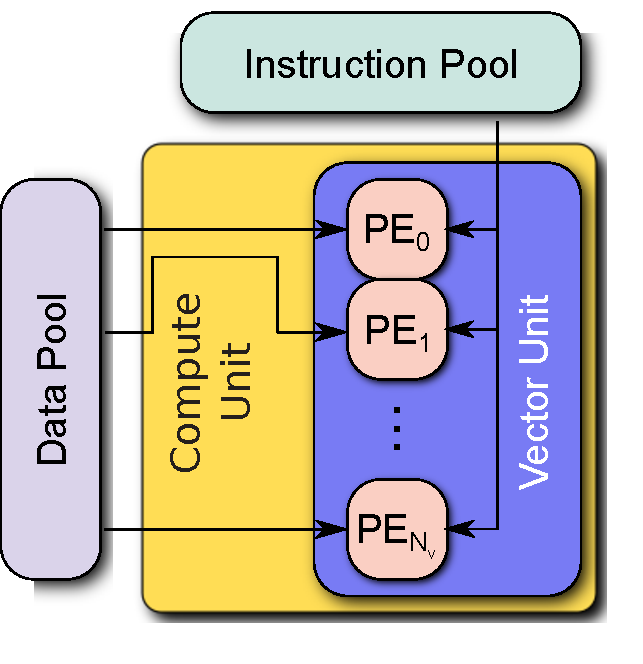
\includegraphics[width=\textwidth]{SIMD.pdf}
      \caption{Schematic of SIMD processing.  A single compute unit (e.g., a CPU core) contains a vector unit with $N_v$ processing elements, together called a vector-lane.  The vector unit executes a single instruction concurrently on multiple data.}
      \label{F:SIMD}
  \end{subfigure}
  \hfill
  \begin{subfigure}[htp]{0.45\linewidth}
      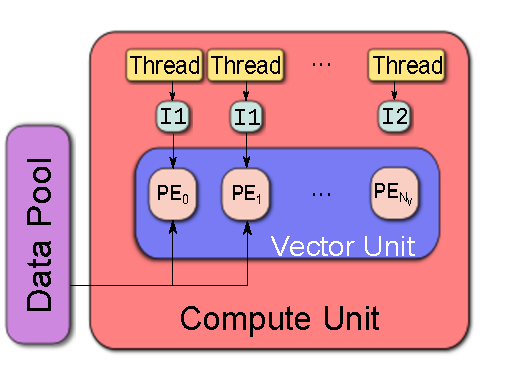
\includegraphics[width=\textwidth]{SIMT.pdf}
      \caption{Schematic of SIMT processing. A single compute unit (e.g., a GPU streaming multiprocessor) contains many processing elements and hosts many threads, each with an instruction to execute (I1, I2).  Threads with the same instruction execute concurrently on multiple data while the others must wait (leading to thread divergence).}
      \label{F:SIMT}
  \end{subfigure}
\end{figure}

A typical modern CPU has many compute units (i.e., cores), each with specialized vector processing units capable of running SIMD instructions (\cref{F:SIMD}).
A SIMD instruction utilizes the vector processor to execute the same floating point operation (e.g. multiplication, division, etc.) on a several different data concurrently; the number of concurrent operations possible is known as the vector-width\footnote{OpenCL allows for use of vector-widths different from the actual hardware vector-width via implicit conversion, and may provide some performance benefit as will be studied in Sec.~\ref{S:results}} and is typically around 2--4 double precision operations. 
Additionally, specialized hardware accelerators, e.g. Intel's Xeon Phi co-processor (MIC) have been developed that have tens of cores with very wide vector-widths (e.g. 4--8 double precision operations); these very wide vector-widths are also expected on cutting-edge and forthcoming Intel CPUs (the Skylake Xeon and Cannon Lake architectures).

SIMT processing---the foundation of modern GPUs~\cite{lindholm2008nvidia}---is a related computing paradigm that hosts large groups of threads on a single compute element (a streaming multiprocessor in NVIDIA terminology).
A group of threads---typically \num{32} threads, known as a warp on NVIDIA GPUs---execute the same SIMD instruction on multiple data concurrently (\cref{F:SIMT}).
If some threads must execute a different instruction---e.g., due to if\slash then branching or predication---they are forced to wait and execute later.
This phenomena, known as thread-divergence, is a key consideration for SIMT-processing and can cause serious performance degradation for complicated algorithms~\cite{CurtisGPU:2017}.

\subsection{Previous works and goals of this study}
Several recent works, e.g.~\cite{CurtisGPU:2017}, have investigated SIMT-based chemical kinetic integration on GPUs, however SIMD-based chemical kinetics have been less studied in comparison.
Stone et al., \cite{stone2016} implemented a linearly-implicit fourth-order stiff Rosenbrock solver in the OpenCL for various platforms including CPUs, GPUs, and MICs.
The shallow-SIMD and SIMT-vectorization models were implemented in OpenCL and compared to an OpenMP baseline code that was deep SIMD-vectorized by simple compiler hints (a.k.a pragmas).
The shallow-SIMD vectorization improved the integrator performance over the OpenMP baseline by \SIrange{2.5}{2.8}{$\times$} on the CPU and \SIrange{4.7}{4.9}{$\times$} on the MIC, while the GPU performance was \SIrange{1.4}{1.6}{$\times$} slower than the OpenMP baseline due to thread-divergence concerns.
\cite{kroshko2013efficient} implemented a shallow-SIMD vectorized third order stiff Rosenbrock integrator for atmospheric chemistry on a Cell Broadband Engine---a specially designed vector processor---finding a speedup of \SI{1.89}{$\times$} over a serial version of the same code.

This work will study the performance of thermo-chemical source term evaluation of automatically generated shallow-SIMD vectorized codes for a wide range chemical kinetic models on the CPU.
The performance will be compared to a baseline shallow-SIMT vectorized code to determine the effective SIMD speedup.
Finally future extensions to this work will be detailed.

\section{Methodology}
\subsection{Data ordering and vectorization patterns}
\label{S:data}

\begin{figure}[htb]
  \centering
  \begin{minipage}{0.45\linewidth}
    \begin{subfigure}[t]{\textwidth}
      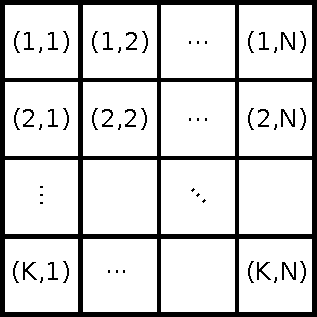
\includegraphics[width=\textwidth]{data_layouts.pdf}
      \caption{A simple 2-D data array with K rows and N columns.}
      \label{F:mem}
    \end{subfigure}
  \end{minipage}
  \hfil
  \begin{minipage}{0.45\linewidth}
    \begin{subfigure}[t]{\textwidth}
	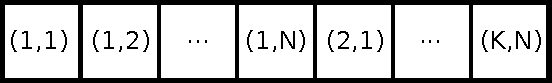
\includegraphics[width=\textwidth]{row_major.pdf}
	\caption{Row-major data ordering}
	\label{F:row_major}
    \end{subfigure}
    \\
    \begin{subfigure}[t]{\textwidth}
	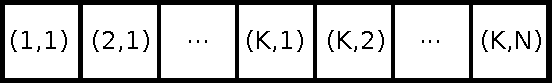
\includegraphics[width=\textwidth]{column_major.pdf}
	\caption{Column-major data ordering}
	\label{F:column_major}
    \end{subfigure}
  \end{minipage}
\end{figure}

When storing arrays for a chemical kinetic model, the data-storage layout and vectorization patterns are critical to achieving high-performance code.
\Cref{F:mem} depicts an example data array with K-rows and N-columns and index (i, j) corresponding to the $i$th row and $j$th column.
For example the concentration of species $j$ for the $i$-th thermo-chemical state would be stored in $[C]_{i, j}$ with $1 \le i \le N_{state}$, the number of thermo-chemical states considered, and $1 \le j \le \ns$, the number of species in the model.
The stored concentrations would then have $K = N_{\text{state}}$ rows, and $N = N_{\text{sp}}$ columns.

In the ``C'' (C row-major) format, the concentrations of all species for a single thermo-chemical condition $i$ would be stored sequentially in memory, i.e., with  $[C]_{1, 1}$ in index \num{1}, $[C]_{1, 2}$ in index \num{2} etc. as shown in \cref{F:row_major}.
Conversely in the ``F'' (Fortran column-major) format, the concentrations of a single species $j$ over all thermo-chemical states are adjacent in memory, corresponding to storing $[C]_{1, 1}$ in index \num{1}, $[C]_{2, 1}$ in index \num{2} and so on, as shown in \cref{F:column_major}.
This ordering---along with the device (CPU, GPU, etc.) and vectorization pattern in question---have a large effect on the performance of SIMD\slash SIMT-vectorized algorithms.

In a \textit{shallow}-SIMD\slash SIMT vectorization, each SIMD-lane (or SIMT-thread) in a compute-unit evaluates thermo-chemical source terms for a different thermo-chemical state.
If the data is stored in ``F''-order, the SIMD-lanes\slash SIMT-thread accessing $[C]_{1, j}\ldots[C]_{L, j})$, the concentration of species $j$ for states $1, 2,\ldots L$---the size of the vector lane for SIMD or the number of threads in a SIMT warp---will load sequential locations in memory, however the first $(j+1)$th species concentration, $[C]_{1, j+1}$ will be $N_{\text{state}}$ memory locations away; this increases the likelihood of cache-misses on the CPU~\cite{gray2000rules}, but conversely is well suited to coalesced memory accesses on the GPU~\cite{NVIDIA:2018}.
In a \textit{deep}-SIMD\slash SIMT vectorization, a compute-unit utilizes its SIMD-lanes\slash SIMT-threads cooperatively to evaluate the thermo-chemical source terms for a single thermo-chemical state, thus SIMD-lanes loading $[C]_{1, j} \ldots [C]_{1, j + L}$---the species concentrations for state 1, species $j \ldots j + L$---will access sequential memory locations if the data is stored in ``C''-order.
Further, in the ``C''-ordering the furthest difference between any two species concentrations within the same thermo-chemical state is at most $N_{\text{sp}}$, with $N_{\text{sp}} \ll N_{\text{state}}$ in most cases; this greatly improved data-locality increases the chances of a cache-hit on the CPU, but leads to uncoalesced memory-accesses on the GPU.
However, a deep vectorization requires both synchronization between SIMD-lanes\slash SIMT-threads, and may result in SIMD-waste\slash SIMT thread-divergence, caused by different SIMD-lanes\slash SIMT-threads executing different instructions (e.g. resulting from different if\slash then branches)

\begin{figure}[htb]
  \centering
  \begin{minipage}{0.6\linewidth}
    \begin{subfigure}[t]{\textwidth}
	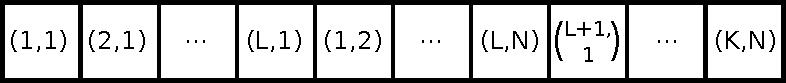
\includegraphics[width=\textwidth]{row_major_split.pdf}
	\caption{Row-major, wide-vectorized data ordering}
	\label{F:row_major_split}
    \end{subfigure}
    \\
    \begin{subfigure}[t]{\textwidth}
	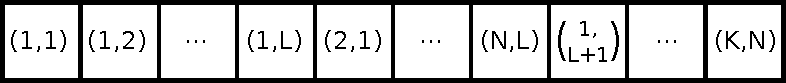
\includegraphics[width=\textwidth]{column_major_split.pdf}
	\caption{Column-major, deep-vectorized data ordering}
	\label{F:column_major_split}
    \end{subfigure}
  \end{minipage}
  \caption{Vectorized data ordering patterns}
  \label{F:vector_data}
\end{figure}

Finally,~\cref{F:vector_data} shows a vectorized data-ordering that improves the caching patterns of a shallow, ``C''-ordered SIMD vectorization on the CPU (\cref{F:row_major_split}) and a deep, ``F''-ordered SIMT vectorization on the GPU (\cref{F:column_major_split}).
This is accomplished by splitting the slower-varying axis of the data array---rows for ``C''-ordering, and columns for ``F''-ordering---into chunks of size $L$ (the SIMD vector-width, or SIMT warp-size) and laying these data out contigously in memory.
For example, using the data-ordering in~\cref{F:row_major_split}, the concentration of species $j$ for states $i\ldots i+L$, $[C]_{i, j} \ldots [C]_{i + L, j}$, are contiguous in memory and are followed by the concentration of species $j + 1$ for the same states, $[C]_{i, j + 1} \ldots [C]_{i + L, j + 1}$.
This pattern, similar to OpenCL's native vector data-types---e.g., \texttt{double\num{8}} which treats \num{8} contiguous double precision floating point numbers as a single vector datum---ensures that any SIMD operation occurs on data that is contiguous in memory, greatly improving caching and SIMD-throughput.
Conversely, the data-ordering in~\cref{F:column_major_split} is designed to enable coalesced memory accesses for ``F''-ordered, deep-SIMT vectorization on the GPU.
The effects of these various data-ordering and vectorization patterns on performance will be studied in~\cref{S:results}.

\subsection{Thermo-chemical Source Terms and Jacobian}
This new version of \texttt{pyJac} is capable of evaluating the thermo-chemical source terms for using both the constant-pressure (\conp) or constant-volume (\conv) assumption\footnote{Note: in this context, the ``constant-pressure'' and ``constant-volume'' assumptions refer to evaluation within a reaction sub-step in the operator splitting scheme, rather than a general constant-pressure or constant-volume reactive-flow simulation.}
In this section, we will only outline a brief summary of the system evaluated by \texttt{pyJac}; the interested reader is referred to our complete derivations, attached as supplimental material to this document.

The thermo-chemical state vector derivation consists of the temperature, the non-constant thermodynamic state parameter (volume or pressure) and the number of moles of all species except the last in the chemical model which is typically taken to be the bath-gas (e.g., \ce{N2}):
\begin{subequations}
\begin{align}
\Phi &= \left\{T, V, n_1, n_2 \ldots n_{\ns - 1}\right\}&\text{\dconp}\\
\Phi &= \left\{T, P, n_1, n_2 \ldots n_{\ns - 1}\right\}&\text{\dconv}
\end{align}
\end{subequations}
where $T$ is the temperature, $V$ and $P$ the volume and pressure respectively, and $n_j$ the number of moles of the $j$th species in the model (containing $\ns$ total species).

For both \conp~and \conv, the molar source terms are~\cite{TurnsStephenR2012Aitc}:
\begin{equation}
\frac{\text{d} n }{\text{d} t }_{k} = V \dot{\omega}_{k} \qquad k = 1, \ldots, \ns - 1, \label{e:spec}
\end{equation}
where $\dot{\omega}_k$ is the $kth$ species' overall production rate, and the temperature production rate~\cite{TurnsStephenR2012Aitc} is:
\begin{subequations}
\label{e:temperature_incomplete}
\begin{align}
\frac{\text{d} T }{\text{d} t } &= - \frac{\sum_{k=1}^{\ns} H_{k} \dot{\omega}_{k}}{\sum_{k=1}^{\ns} [C]_{k} {C_{p, k}}} & \text{\dconp} \\
\frac{\text{d} T }{\text{d} t } &= - \frac{\sum_{k=1}^{\ns} U_{k} \dot{\omega}_{k}}{\sum_{k=1}^{\ns} [C]_{k} {C_{v, k}}} & \text{\dconv}
\end{align}
\end{subequations}
where $H_k$, $U_k$, $C_{p,k}$ and $C_{v, k}$ are the enthalpy, internal energy, constant-pressure and constant-volume specific heat of species $k$ in molar units respectively, while $[C]_{k}$ is the concentration, given by:
\begin{equation}
 [C]_{k} = \frac{n_{k}}{V}
\end{equation}
By differentiating the ideal gas law, the volume and pressure source terms can be found:
\begin{subequations}
\label{e:param_complete}
\begin{align}
\frac{\text{d} V }{\text{d} t } &= V \left(\frac{T \Ru}{P} \sum_{k=1}^{\ns  - 1} \left(1 - \frac{W_{k}}{W_{\ns}}\right) \dot{\omega}_{k} + \frac{1}{T} \frac{\text{d} T }{\text{d} t }\right)& \text{\dconp} \\
\frac{\text{d} P }{\text{d} t } &= T \Ru \sum_{k=1}^{\ns  - 1} \left(1 - \frac{W_{k}}{W_{\ns}}\right) \dot{\omega}_{k} + \frac{P}{T} \frac{\text{d} T }{\text{d} t }&\text{\dconv}
\end{align}
\end{subequations}
where $\mathcal{R}$ is the ideal gas-constant.

\subsection{Code Generation}
Code generation is enabled by the python package \texttt{loo.py}~\cite{kloeckner_loopy_2014}, which translates user specified psuedo-code and data to OpenCL, allowing for unit testing and easy changes of program structure, e.g. data ordering, vectorization, threading patterns etc.

\section{Results and Discussion}
\subsection{Comparison to Cantera}
The reaction rates of progress (ROP), species and temperature rates in this study are validated by comparison with Cantera~\cite{Cantera}, however special care must be taken due floating point arithmetic issues.

For a direct comparison, a relative error norm of a quantity $X_{ij}$ over all states $j$, and reactions (or species) $i$ was computed using the $L^{\infty}$ norm:
\begin{equation}
E_{X} = \left\lVert \frac{\left\lvert X_{ij,\text{CT}} - X_{ij}\right\rvert}{\num{e-10} + \num{e-6} * \left\lvert X_{ij,\text{CT}} \right\rvert} \right\rVert_{i,j,\infty}
\label{e:rel_err}
\end{equation}
where the \text{CT} subscript indicates values from Cantera~\cite{Cantera}

However, in computing the net ROP of reaction $i$ for state $j$ from the forward and reverse ROP: $R_{ij} = R_{ij}^{\prime} - R_{ij}^{\prime\prime}$, accuracy can easily be lost as the net ROP may be---particularly near chemical equilibrium---many orders of magnitude smaller than the forward or reverse rates.
To quantify this phenomena, the error in forward ROP is first defined as:
\begin{equation}
\varepsilon^{\prime}_{ij} = \left\lvert R_{ij}^{\prime} - R_{ij,\text{CT}}^{\prime} \right\rvert
\end{equation}
while the error in reverse ROP, $\varepsilon^{\prime\prime}_{ij}$, can be defined analogously.
Finally, for the reaction $i^{*}$ and state $j^{*}$ that result in the largest error in net ROP, i.e. $E_{R}$, an estimate of the error attributable to floating point error accumulation from the forward and reverse ROPs can be obtained as:
\begin{equation}
E_{\varepsilon} = \frac{\max(\varepsilon^{\prime}_{i^{*}j^{*}}\text{, }\varepsilon^{\prime\prime}_{i^{*}j^{*}})}{\num{e-10} + \num{e-6} * \left\lvert R_{i^{*}j^{*},\text{CT}} \right\rvert}
\end{equation}
This estimate allows for direct comparison of the error in forward or reverse ROPs to the value of the net ROP itself, if they are of similar magnitude the error in net ROP will be large.

\begin{table}[htb]
\sisetup{retain-zero-exponent=true}
\centering
\begin{tabular}{@{}S[table-format=1.2e1] S[table-format=1.2e1] S[table-format=1.2e1] S[table-format=1.2e1] S[table-format=1.2e1] S[table-format=1.2e1] S[table-format=1.2e1] @{}}
\toprule
\multicolumn{1}{l}{Model} & \multicolumn{1}{c}{$E_{R^{\prime}}$} & \multicolumn{1}{c}{$E_{R^{\prime\prime}}$} &\multicolumn{1}{c}{$E_{R}$} & \multicolumn{1}{c}{$E_{\varepsilon}$} & \multicolumn{1}{c}{$E_{\dot{\omega}}$} & \multicolumn{1}{c}{$E_{\frac{\partial T}{\partial t}}$} \\
\midrule
\multicolumn{1}{l}{\ce{H2}\slash~\ce{CO}\cite{Burke:2011fh}} & 1.20e-8 & 6.33e-8 & 1.32e1 & 1.32e1 & 2.37e1 & 2.12e5 \\
\multicolumn{1}{l}{GRI-Mech.~3.0\cite{smith_gri-mech_30}}  & 3.11e-8 & 5.90e-8 & 1.21e0 & 1.29e0 & 2.84e0 & 2.64e4 \\
\multicolumn{1}{l}{USC-Mech II\cite{Wang:2007}}  & 1.07e-7 & 1.37e-7 & 2.39e0 & 2.27e0 & 7.92e0 & 3.22e03 \\
\multicolumn{1}{l}{\ce{iC5H11OH}\cite{Sarathy:2013jr}} & 6.80e-8 &  1.48e-7 & 5.26e-1 & 4.87e-1 & 2.26e00 & 6.10e+01 \\
\bottomrule
\end{tabular}
\caption{Summary of rate of progress, species and temperature rate correctness.
Error statistics are based on the infinity-norm of the relative error detailed in Eq.~\eqref{e:rel_err} for each quantity.
}
\label{T:error}
\end{table}

In Table~\ref{T:error}, we see the results of this code as compared to Cantera~\cite{Cantera} on a library of partially stirred reaction conditions (PaSR) described in our previous works~\cite{CurtisGPU:2017,Niemeyer:2016aa}.
Very close agreement is observed for the forward and reverse ROP for all models, however the net ROP error norm is \numrange{7}{9} orders of magnitude larger.
We see here that $E_{\varepsilon}$ is very similar in magnitude to $E_R$ in all cases, indicating that this large increase in error is caused by the accumulation of floating point error from the forward and reverse ROPs, as previously discussed.
The species rate error norm is similar in magnitude to that of the net ROP, however the temperature rate error again increases as the error in species rates is amplified by multiplication with thermodynamic properties.
We note that the above discussion does not imply that computation of the net ROP will cause large error in chemical kinetic integration---either in this code or Cantera~\cite{Cantera}---as this loss of accuracy only occurs when the forward and reverse ROP are nearly equal, implying the reaction is in near-equilibrium.

\subsection{Performance}
\label{S:results}
The performance studies in this work were run on four ten-core \SI{2.2}{\giga\hertz} Intel Xeon E5-4640 v2 CPUs with \SI{20}{\mega\byte} of L3 cache memory, installed on an Ace Powerworks PW8027R-TRF+ with a Supermicro X9QR7-TF+/X9QRi-F+ baseboard.
Runtimes in each case were averaged over ten runs, each using the same set of PaSR conditions utilized in validation.
All code was compiled with \texttt{gcc 4.8.5} and ``\texttt{-O3}'' optimization, running on \texttt{v16.1.1} of the Intel OpenCL runtime supporting OpenCL \texttt{v1.2}.

\begin{figure}[htb]
  \centering
  \begin{minipage}[t]{0.48\linewidth}
    \includegraphics[width=\textwidth]{SIMD_SIMT_Order_comparison}
    \caption{Runtime in milliseconds per thermo-chemical state of shallow-SIMD and SIMT-vectorization on a single CPU core for both ``C'' (filled symbols) and ``F'' (empty symbols) data ordering.}
    \label{F:SIMDComp}
  \end{minipage}
  \hfill
  \begin{minipage}[t]{0.48\linewidth}
    \includegraphics[width=\textwidth]{SIMD_Vecwidth_comparison}
    \caption{Speedup of a ``C''-ordered shallow-SIMD vectorization on a single CPU core when varying the supplied vector-width.}
    \label{F:Veccomp}
  \end{minipage}
\end{figure}
\begin{figure}[htb]
  \centering
  \begin{minipage}[t]{0.5\linewidth}
    \includegraphics[width=\textwidth]{SIMD_scaling}
    \caption{Strong parallel scaling efficiency of a ``C''-ordered shallow-SIMD vectorization using a vector-width of 16.}
    \label{F:SIMDscale}
  \end{minipage}
\end{figure}


In Fig.~\ref{F:SIMDComp}, the performance of the shallow-SIMD and SIMT vectorization are compared on a single CPU core for both ``C'' and ``F'' memory formats.
The ``C''-ordered SIMD\slash SIMT vectorizations show a speedup over the equivalent ``F''-ordered code by \SIrange{1.46}{2.00}{$\times$} and \SIrange{1.61}{2.38}{$\times$} respectively.
This demonstrates that enhanced data-locality of the ``C''-ordering for CPU caching---discussed in Sec.~\ref{S:data}---is key to high performance on the CPU, and suggests that a deep vectorization would see even greater accelerations.
The shallow vectorization is consistently faster than the SIMT vectorization, by \SIrange{1.73}{1.90}{$\times$} and \SIrange{2.00}{2.45}{$\times$} for the ``C'' and ``F'' memory formats respectively.
This is less than the theoretical maximum speedup on this CPU, which can process \SI{256}{\bit} AVX instructions (i.e. four double-precision operations) concurrently.
Most likely this is due to the non-sequential memory access patterns of the shallow vectorization discussed previously, but could also be caused in part by inefficiencies in translation of the OpenCL code to AVX code, a process handled by the Intel Opencl Runtime.

The effect of changing the vector-width supplied to a ``C''-ordered shallow-SIMD vectorization on a single CPU core is investigated in Fig.~\ref{F:Veccomp}.
Significant speedups are seen with larger vector-widths for the smaller models, however as the model size increases data must be loaded from increasingly distant memory locations and the performance of all three vector-widths becomes similar.

Finally, the strong parallel scaling efficiency is defined as:
\begin{equation}
S = \frac{t_1}{N t_N}
\end{equation}
where $t_1$ is the mean wall-clock runtime of thermo-chemical source terms evaluation on one core and $t_N$ the mean runtime on $N$ cores.
Fig.~\ref{F:SIMDscale} examines the strong parallel scaling efficiency for all four models with a ``C''-ordered shallow SIMD-vectorization and vector-width of 16.
Interestingly the efficiency of the hydrogen model decreases the fastest while the larger models have significantly larger scaling efficiencies for more than 4 cores.
Additionally, it appears that for a fixed number of cores, the scaling efficiency increases with model size.
This suggests that evaluation of the chemical-source terms for a single thermo-chemical state for the smaller models may not saturate the processing power of the CPU, some efficiency may be lost due to context switching within OpenCL itself.
Additionally, OpenCL allows assigning of work to devices by shared memory resources, e.g., a L3 cache, which was not pursued in this study for simplicity; this should be investigated in future work to determine the effect on scaling efficiency.

\section{Conclusions}
In this work, automatically generated OpenCL codes for shallow SIMD-vectorized thermo-chemical source term evaluation were developed and validated against Cantera~\cite{Cantera} for a wide range of chemical kinetic models~\cite{Burke:2011fh,smith_gri-mech_30,Wang:2007,Sarathy:2013jr}.
Significant speedups of up to \SIrange{1.90}{2.45}{$\times$} over a baseline SIMT-vectorized code were observed.
Two data-ordering schemes were investigated, showing a clear performance benefit for use of the ``C'' (row-major) ordering for the shallow vectorized code.
Further, this study suggests that a deep SIMD-vectorized code---currently under development---may see even greater accelerations due to expected increases in cache-hit rates.
Larger vector-widths were found to provide accelerations for the smaller models studied, but the speedup was similar over all vector-widths tested for the largest models investigated.
Finally, the strong parallel scaling efficiency was examined for the shallow vectorized code; the larger models exhibited higher scaling efficiency, possibly due to failure of the \ce{H2}\slash\ce{CO} model to saturate the CPU throughput.
Future extensions of this work will include development of a SIMD\slash SIMT-accelerated sparse-analytical Jacobian code targeted at CPUs, GPUs, and MICs.

\section{Acknowledgements}
This research was funded by the National Science Foundation under grant ACI-1534688.

\bibliography{paper}

\end{document}
